\section{System Design}

The system of the validator nodes and their supporting components are designed to provide security and stability. The basic layout is shown in Figure ~\ref{fig:sysdesign}.
Also along the active validator set is a set of standby validator nodes called Shadow Validators, that can swap in for any failed or otherwise compromised validator.

\begin{figure}[ht]
	\centering
    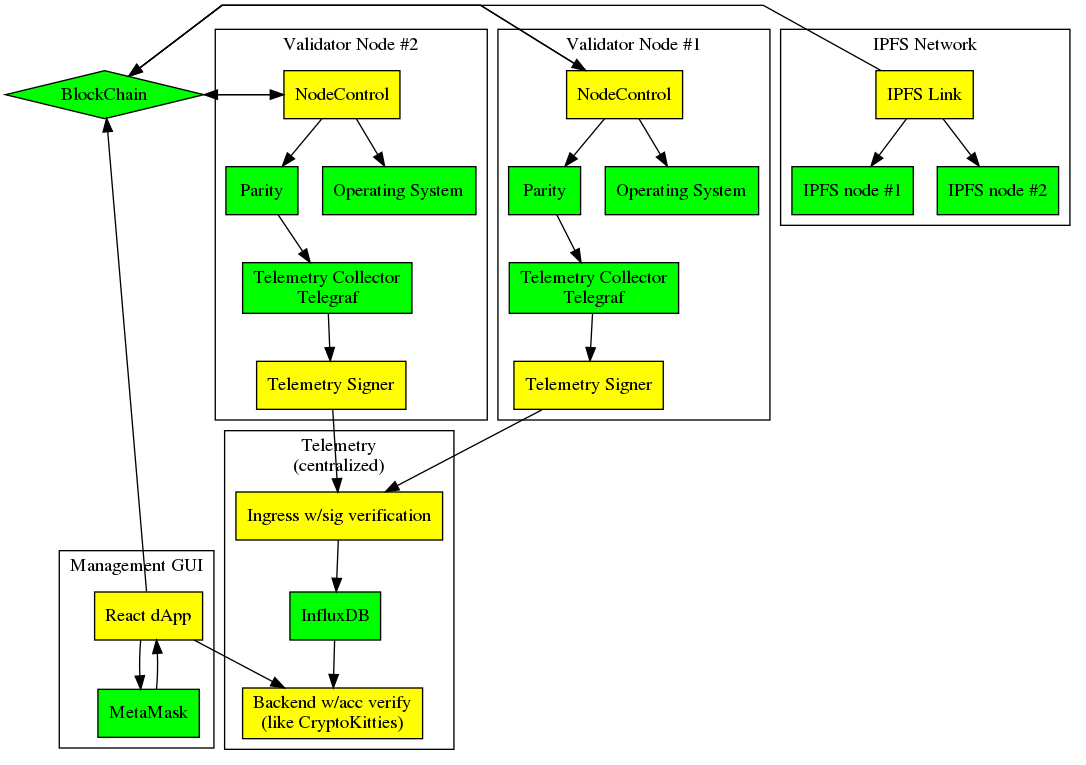
\includegraphics[width=0.85\textwidth,keepaspectratio]{./images/sys-diagram.png}
	\caption{Validator System Design}
	\label{fig:sysdesign}
\end{figure}

\subsection{Shadow Validators [Not part of MVP]}

As running hundreds of validators at the same time increases network traffic and also time to finality a lot, the concept of shadow validators can be used to have a small set of 23 active validators and a number of dormant shadow validators.

During onboarding an affiliate can choose either to run a single validator node or provide resources for two validator nodes from which only one gets enlisted into the active validator set.
The second node is also completely onboarded but would run with the sealer disabled. 
It would be just a normal peer acting as a full node (as any other validator would).
If another validator node would go offline or start misbehaving, the network starts to counteract this behavior by activating a shadow validator, while in the same time remove the misbehaving validator from the active set. This will happen automatically via the validator smart contract. To ensure the network can heal it self this way, the validator address of the shadow node is recorded to the validator contracts shadow node list, from which it then can draw new nodes. The contract will emit a wake up event that will be picked up by NodeControl on the dormant validator node and restarts the blockchain client with the sealer enabled. NodeControl reports back successful activation to the validator contract which then will add the now active shadow node to the active list of validators. Along with the wakeup event a disable event is recorded on chain for the misbehaving one.

The main purpose of this is to counteract single-node attacks, where one node is brought down due to some kind of DoS attack. 
Once the attacked node is back up again and re-validated by NetOps, it can replace the activated shadow node  which then would go back to be dormant. \\

Additional idea is to use this mechanism to swap random nodes in and out of the shadow set on a regular basis. Governance has to make sure that over the period of a year each validator had an equal share of "active time" to evenly distribute transaction fees and block rewards.


\subsection{System Components}
\label{components}

These system components are tailor made or where developed for the validator network.

\subsubsection{NodeControl}

A small deamon that will carry out updates on behalf of NetOps. See \ref{nodecontrol}.

\subsubsection{Telemetry Signer}

System telemetry is collected using Telegraf. But to ship the telemetry, Telegraf won't send it directly to the telemetry backend but instead to a local deamon called "Telemetry Signer".
This deamon will make sure that telemetry is only send to a verified telemetry collection endpoint (Telemetry Ingress) using TLS certificate fingerprints.
Each telemetry package send to the Ingress will be signed by the telemetry signer.

\subsubsection{Telemetry Ingress}

A deamon that will wait for connections from telemetry signers. It will verify the signature of each incoming telemetry package before inserting it into the InfluxDB telemetry datastore. If the signature is not valid it will report this to a log file.

\subsubsection{IPFS Link [Not part of MVP]}

IPFS Link is a service that allows human readable urls to be resolved to IPFS hashes. It is used in this system to provide the link to the NetOps Management dApp. This way the management dApp can be hosted decentralized to increas reliability.

\subsection{Other Components}

These components are standardize open-source components.

\subsubsection{IPFS [Not part of MVP]}

IPFS is used to distribute the management ui. A central support node would provide an IPFS node that is connected to the public IPFS network. The management UI would be accessed either through a local IPFS client or trough a public IPFS gateway.
This way the UI stays accessible, even when the support node fails.

\subsubsection{Telemetry Collector}

The system uses Telegraf to collect the telemetry from on the nodes. This collected data is then send via the InfluxDB wire protocol to the also locally running telemetry signer.

\subsubsection{Grafana [Only MVP]}

To visualize the telemetry the telemetry node will run a Grafana instance. In a later milestone this then could be replaced or integrated into the governance dApp.

\subsubsection{Blockchain Client}

The blockchain client is the main component of the system as it provides the connection to the blockchain and also carries out signing and validation duties. 
The probably used software will be Parity-Ethereum from Parity Tech running the AURA Proof-of-Authority engine.

